\documentclass[11pt]{article}
\usepackage{placeins}
\usepackage{graphicx}
\usepackage{url}

\begin{document}

\begin{titlepage}
	\begin{center}
    	
\includegraphics[scale=0.10]{du.png}\par
		\begin{Huge}
			\textsc{University of Dhaka}\par
		\end{Huge}
		\begin{Large}
			Department of Computer Science and Engineering\par \vspace{.5cm}
			CSE-3111 : Computer Networking Lab \\[12pt]	
			Lab Report 6:Implementation of TCP Reno congestion control algorithm.
		\end{Large}
	\end{center}  	
	\begin{large}
		\textbf{Submitted By:\\[12pt]}
			Name : Tasfia Tabassum\\[8pt]
			Roll No : 24\\[12pt]
			Name : Saima Akter\\[8pt]
			Roll No : 30\\[12pt]
		\textbf{Submitted On : \\[12pt]}
			February 28, 2023\\[20pt]
		\textbf{Submitted To :\\[12pt]}
			Dr. Md. Abdur Razzaque\\[12pt]
                Md Mahmudur Rahman\\[12pt]
                Md. Ashraful Islam\\[12pt]
                Md. Fahim Arefin
	\end{large}
\end{titlepage}

\section{Introduction}
TCP Reno is a widely used congestion control algorithm for TCP/IP networks. It is designed to improve the stability and fairness of TCP flow by detecting and reacting to network congestion in a timely and efficient manner. TCP Reno is based on the principle of congestion avoidance, which involves reducing the transmission rate of TCP connections to prevent congestion before it occurs. This is achieved through a series of mechanisms that include slow start, congestion avoidance, and fast recovery. TCP Reno is one of the most widely implemented congestion control algorithms and is supported by most operating systems and network equipment.

In this project, we will be implementing TCP Reno congestion control algorithm to observe its behavior in a simulated network environment. The goal of this project is to gain a deeper understanding of the TCP Reno algorithm and its behavior under different network conditions. 

\subsection{Objectives}
\begin{itemize}
    \item Our objective is to understand and implement the TCP Reno congestion control algorithm
    
    \item Our goal is to compare TCP Reno with TCP Tahoe

\end{itemize}
%%%%
%%%%
\section{Theory}
TCP Reno is a congestion control algorithm used in the Transmission Control Protocol (TCP) to manage network congestion. It was named after the city of Reno, Nevada, where the algorithm was first presented at a conference in 1990. TCP Reno is an extension of the earlier TCP Tahoe algorithm, and it introduces a new mechanism called "fast recovery" to improve network performance. TCP Reno operates in four phases: slow start, congestion avoidance, fast retransmit, and fast recovery.


\textbf{1. Slow Start:}\\[12pt]  
When a connection is established, the congestion window size is initially set to 1. The window size is increased by 1 for each ACK received, doubling the window size every round trip time (RTT) until the slow start threshold is reached.

\newpage
\textbf{2. Congestion Avoidance:}\\[12pt] 
Once the slow start threshold is reached, the congestion window size is increased linearly, by
1/cwnd for each ACK received, where cwnd is the current congestion window size.

\textbf{3. Fast Retransmit: }\\[12pt]
When three duplicate ACKs are received, TCP Reno assumes that a packet has been lost and immediately retransmits the lost packet.

\textbf{4. Fast Recovery: }\\[12pt]
After retransmitting the lost packet, TCP Reno enters the fast recovery phase. The congestion window size is halved and 3 is added to it, and then kept constant until all lost packets are retransmitted. After that, the congestion avoidance phase is entered, and the congestion window size is increased linearly.


\section{Methodology}

\subsection{Server}
TCP Reno is a variant of the Transmission Control Protocol (TCP) that is widely used in modern computer networks. It is a congestion control algorithm that aims to provide reliable and efficient data transmission over the internet. In order to implement a server using TCP Reno, the following algorithm can be used:
\begin{itemize}
\item The server first creates a TCP socket and binds it to a port number on the local machine.

\item The server then waits for incoming connections from clients. When a client connects, the server accepts the connection and creates a new socket for communication with the client.

\item The server receives data from the client using the newly created socket. It uses the TCP Reno algorithm to control the transmission rate and ensure reliable delivery of the data.

\item If the server receives an acknowledgement (ACK) from the client indicating that the data has been received, it sends the next packet of data to the client.

\item If the server does not receive an ACK within a certain amount of time, it assumes that the packet has been lost and retransmits it.

\item If the server detects congestion on the network, it reduces the transmission rate to avoid further congestion.

\item When the server has finished sending data to the client, it closes the connection by sending a FIN packet to the client.

\item The server then waits for a response from the client indicating that it has received the FIN packet, and when it receives this response, it closes the socket.
\end{itemize}
This algorithm ensures that the server uses the TCP Reno congestion control algorithm to provide reliable and efficient data transmission over the internet. It allows the server to control the transmission rate based on network conditions, and ensures that data is delivered reliably even in the presence of network congestion.


\subsection{Client}
To implement a client using TCP Reno, the following algorithm can be used:
\begin{itemize}
\item The client creates a TCP socket and establishes a connection to the server by specifying the server's IP address and port number.

\item The client sends data to the server using the TCP Reno algorithm to control the transmission rate and ensure reliable delivery of the data.

\item If the client receives an acknowledgement (ACK) from the server indicating that the data has been received, it sends the next packet of data to the server.

\item If the client does not receive an ACK within a certain amount of time, it assumes that the packet has been lost and retransmits it.

\item If the client detects congestion on the network, it reduces the transmission rate to avoid further congestion.

\item When the client has finished sending data to the server, it sends a FIN packet to the server to indicate that it is done.

\item The client then waits for a response from the server indicating that it has received the FIN packet, and when it receives this response, it closes the socket.
\end{itemize}
This algorithm ensures that the client uses the TCP Reno congestion control algorithm to provide reliable and efficient data transmission over the internet. It allows the client to control the transmission rate based on network conditions, and ensures that data is delivered reliably even in the presence of network congestion.


\subsection{Algorithm to implement TCP Reno : }

 \begin{figure}[!h]
\centering
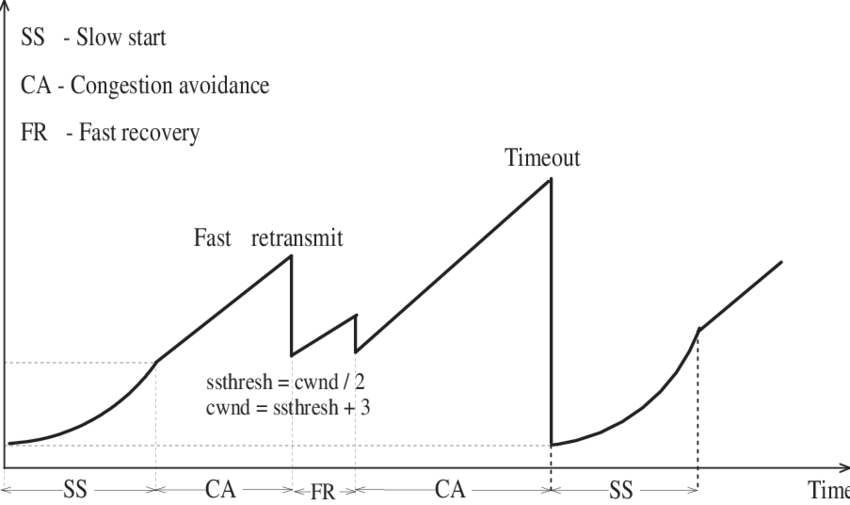
\includegraphics[width=\textwidth]{reno_general.png}
\caption{Graph on TCP Reno}
\end{figure}
\FloatBarrier

The x-axis of the graph represents time, while the y-axis represents the congestion window size (CWND) of the TCP connection. The congestion window size determines how many packets can be sent by the sender before receiving an acknowledgement (ACK) from the receiver.

In the beginning, the congestion window size starts at a small value and gradually increases as the sender sends more packets. However, when congestion is detected in the network, the congestion window size decreases sharply to reduce the rate of packet transmission and prevent further congestion.

Once the network congestion has eased, the congestion window size gradually increases again until it reaches a point where congestion occurs again, and the cycle repeats. This cycle of increasing and decreasing congestion window size continues until the end of the TCP connection.

Overall, TCP Reno aims to balance between high throughput and network congestion avoidance by dynamically adjusting the congestion window size based on network conditions.

\subsubsection{Output for the Server Program}

 \begin{figure}[!h]
\centering
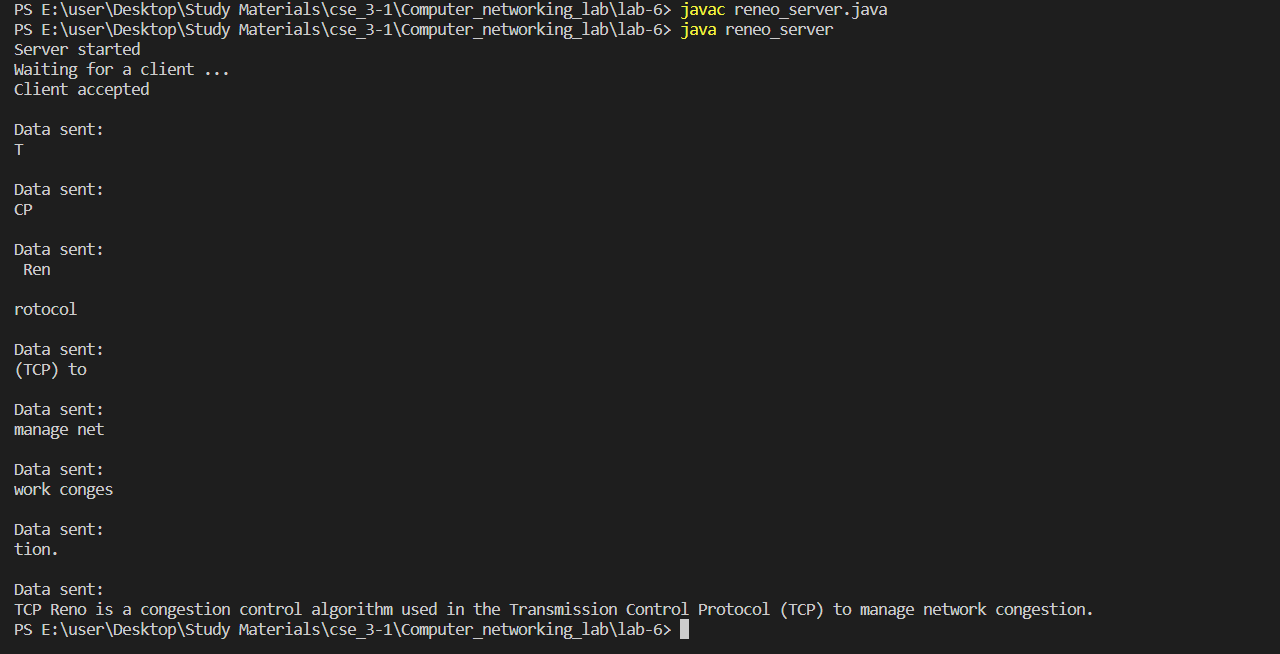
\includegraphics[width=\textwidth]{ren_server.png}
\caption{Terminal output of server java file }
\end{figure}
\FloatBarrier


\subsubsection{Output for the Client Program}

  \begin{figure}[!h]
\centering
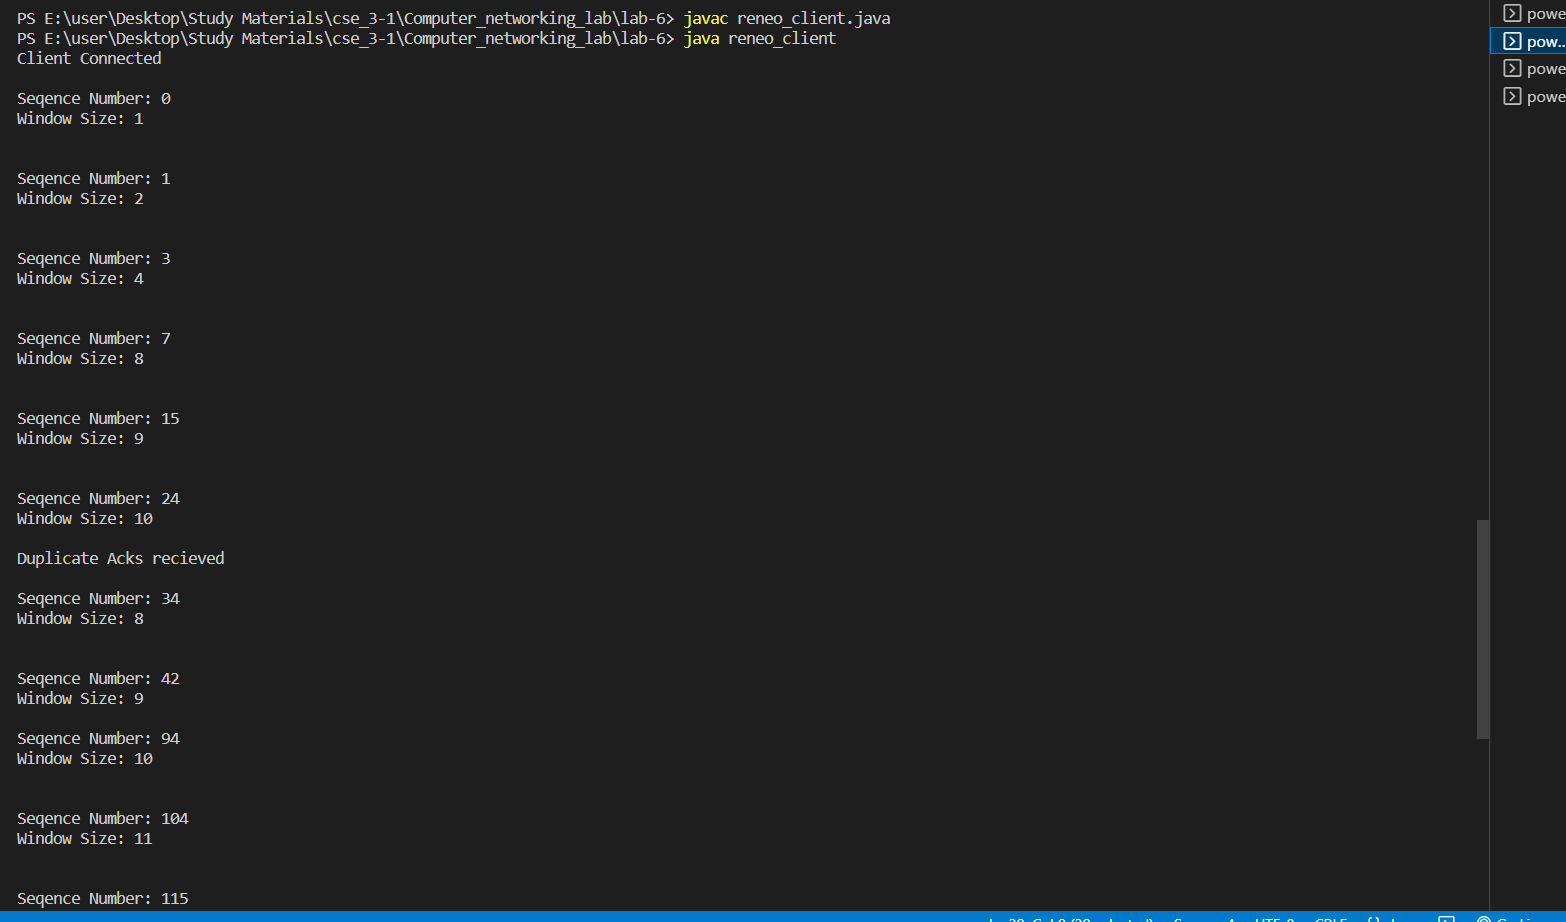
\includegraphics[width=\textwidth]{ren_client1.png}
\caption{Terminal output of client java file }
\end{figure}
\FloatBarrier

 \begin{figure}[!h]
\centering
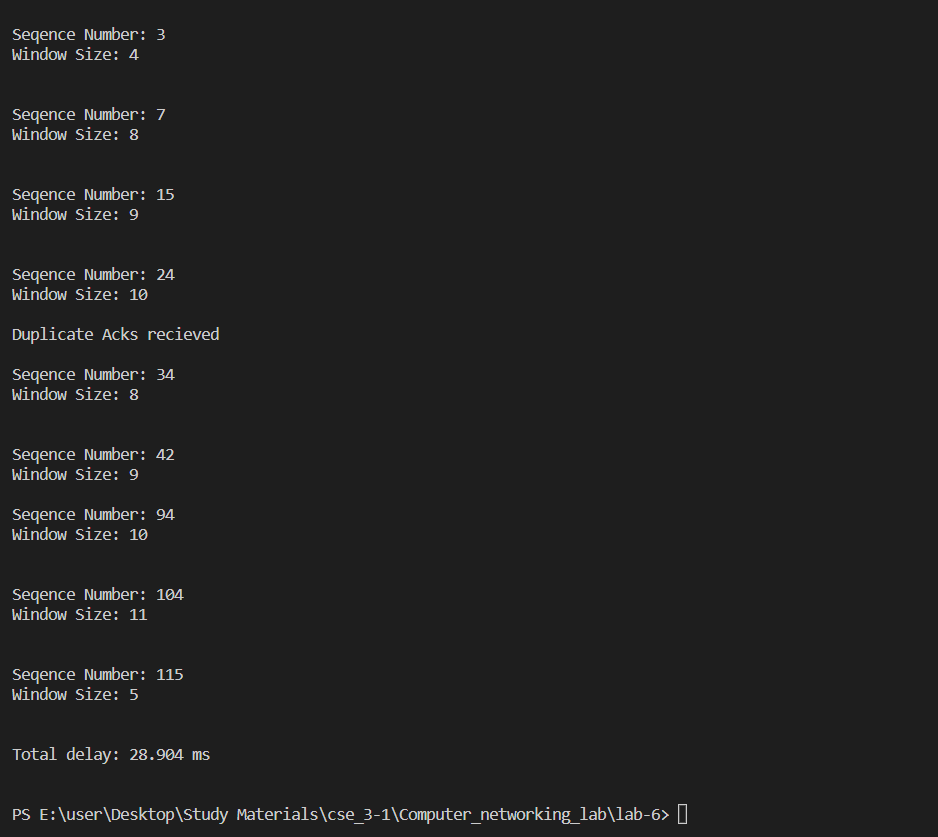
\includegraphics[width=\textwidth]{ren_client2.png}
\caption{Terminal output of client java file }
\end{figure}
\FloatBarrier

\subsection{Output Result for TCP Tahoe :}

\subsubsection{Output for the Server Program}

 \begin{figure}[!h]
\centering
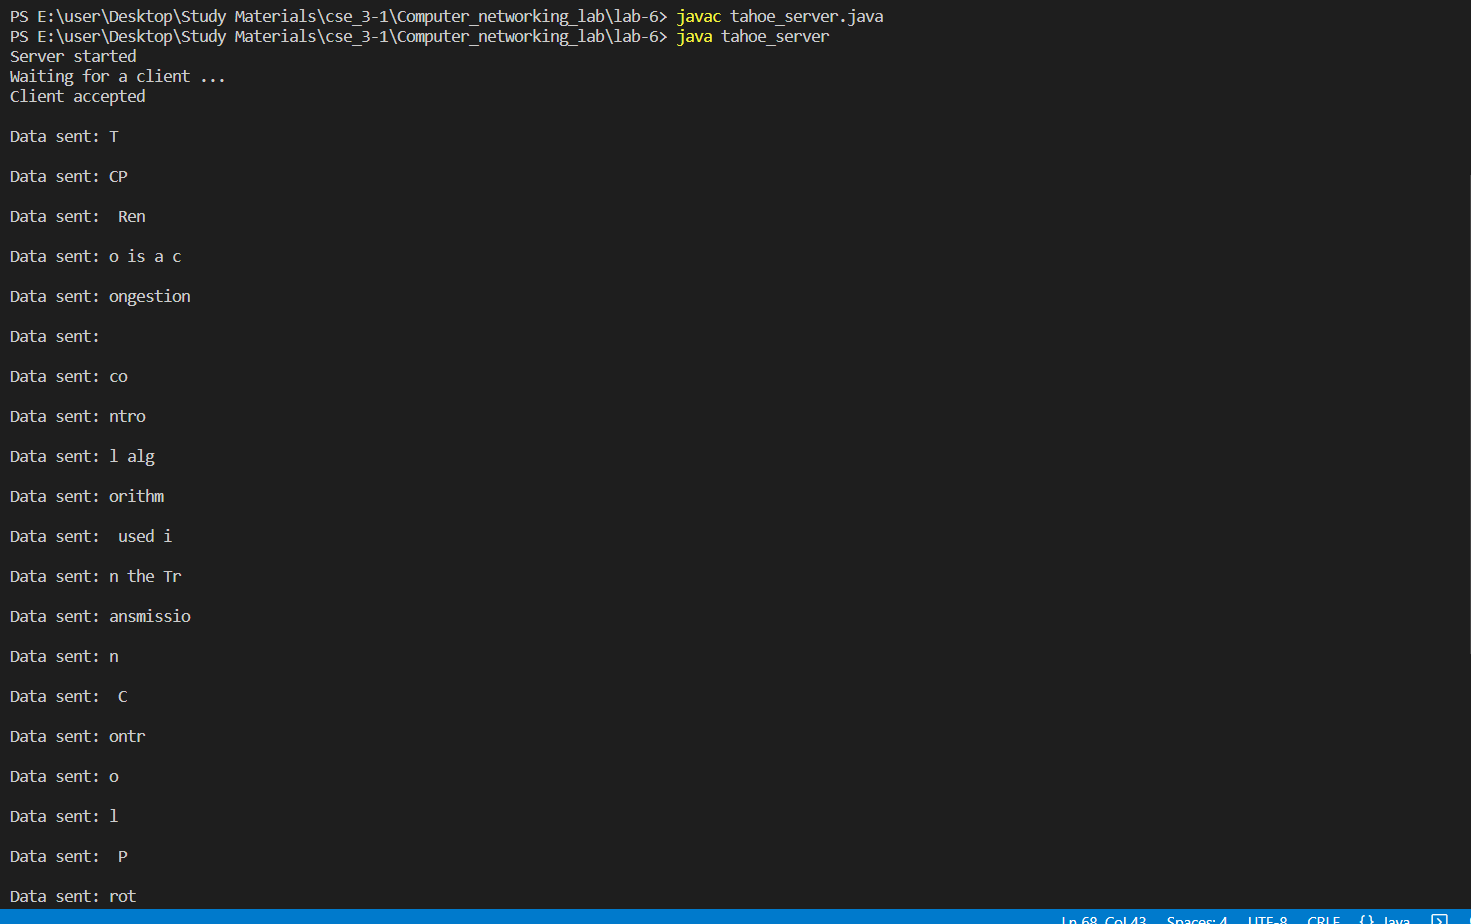
\includegraphics[width=\textwidth]{t_server1.png}
\caption{Terminal output of server java file }
\end{figure}
\FloatBarrier

 \begin{figure}[!h]
\centering
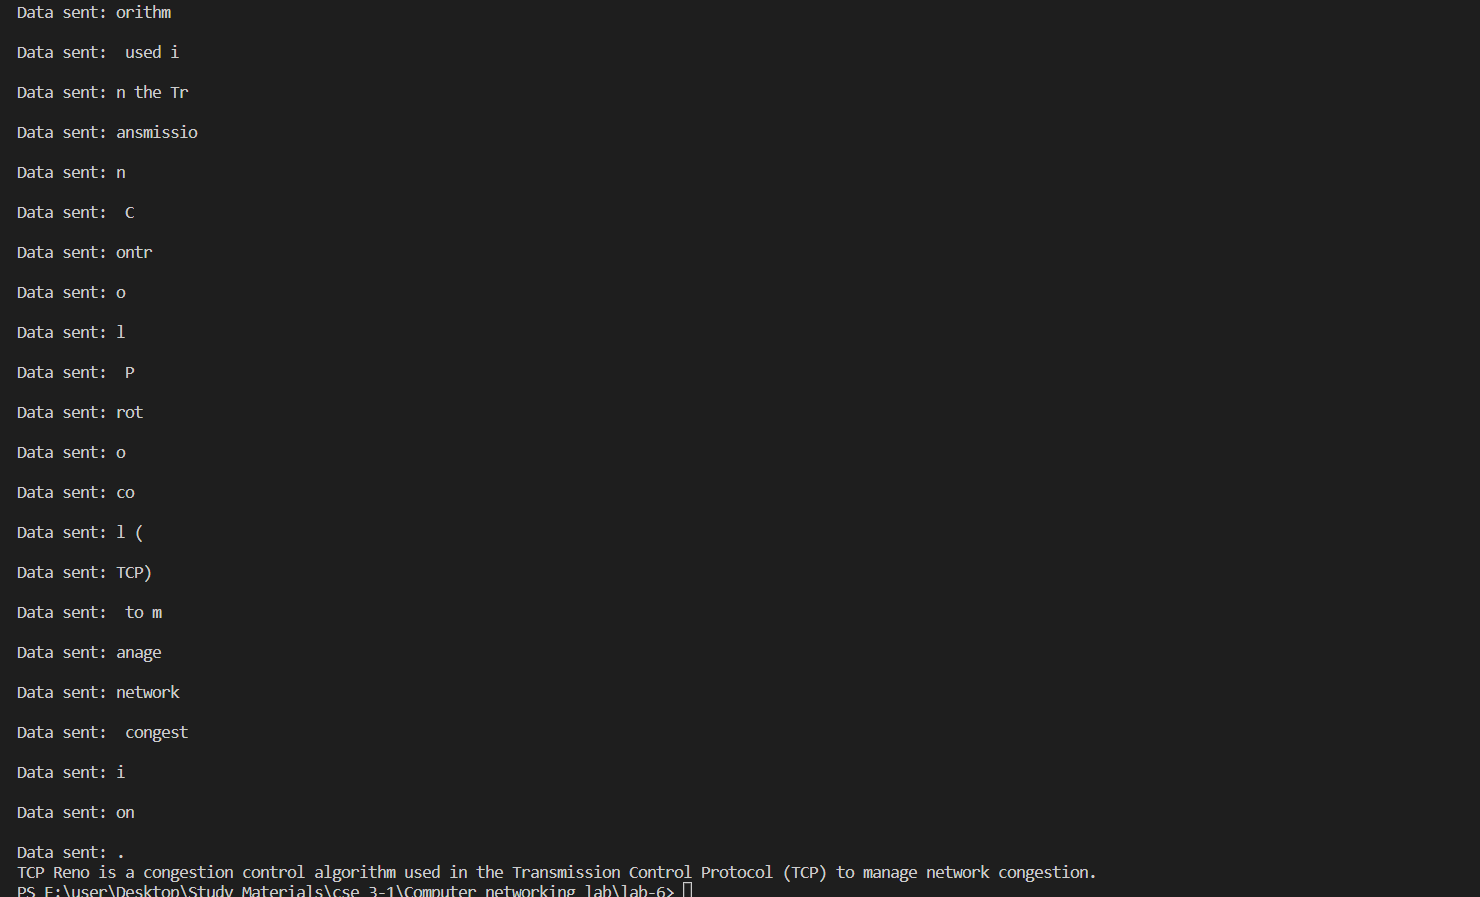
\includegraphics[width=\textwidth]{t_server2.png}
\caption{Terminal output of server java file }
\end{figure}
\FloatBarrier


\subsubsection{Output for the Client Program}

  \begin{figure}[!h]
\centering
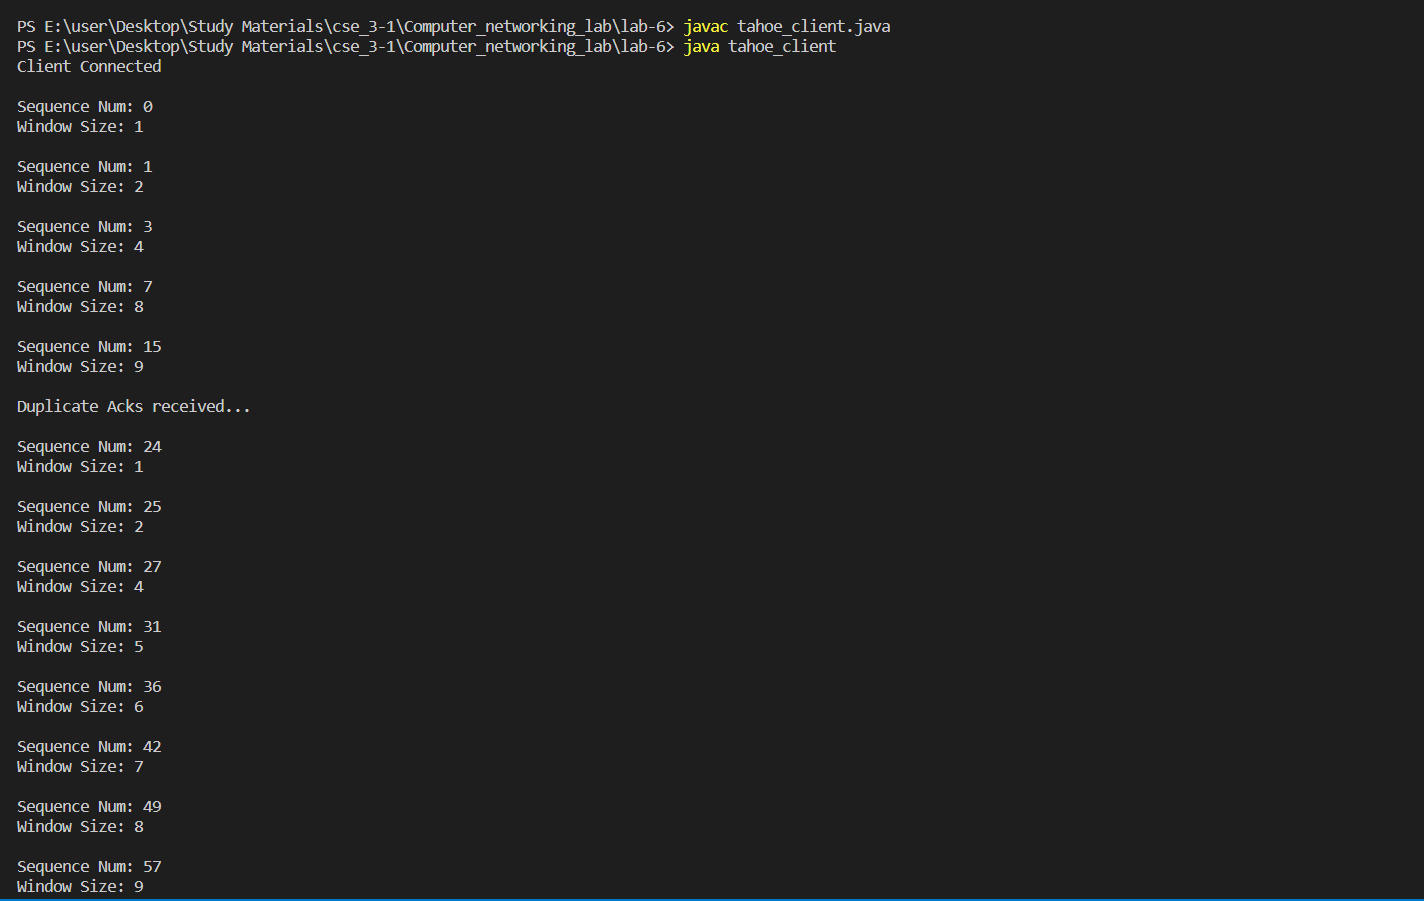
\includegraphics[width=\textwidth]{t_client1.png}
\caption{Terminal output of client java file }
\end{figure}
\FloatBarrier

 \begin{figure}[!h]
\centering
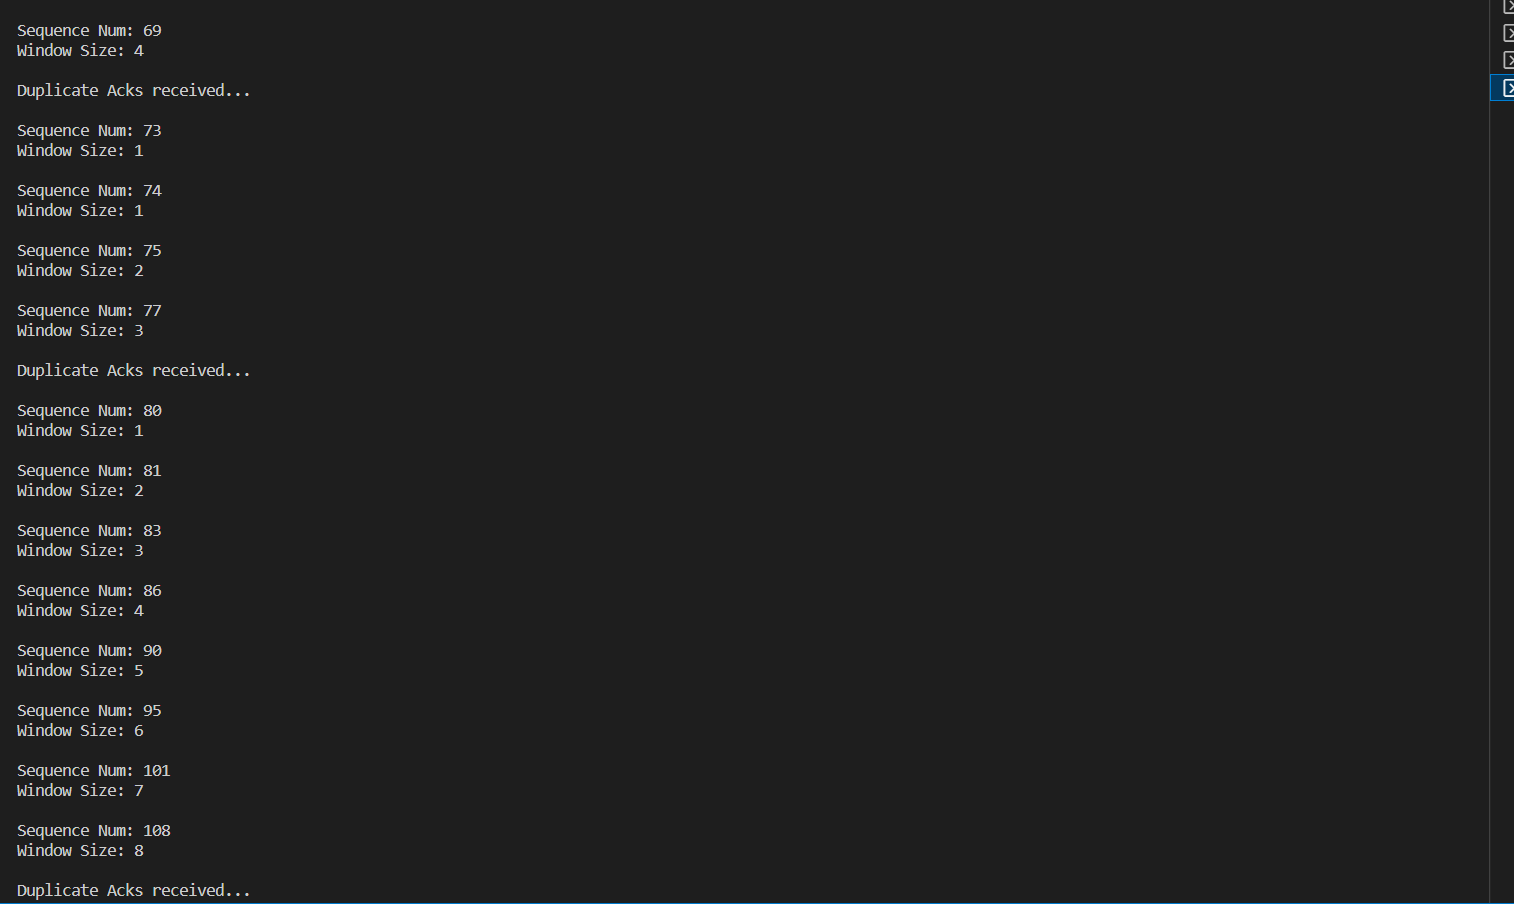
\includegraphics[width=\textwidth]{t_client2.png}
\caption{Terminal output of client java file }
\end{figure}
\FloatBarrier

 \begin{figure}[!h]
\centering
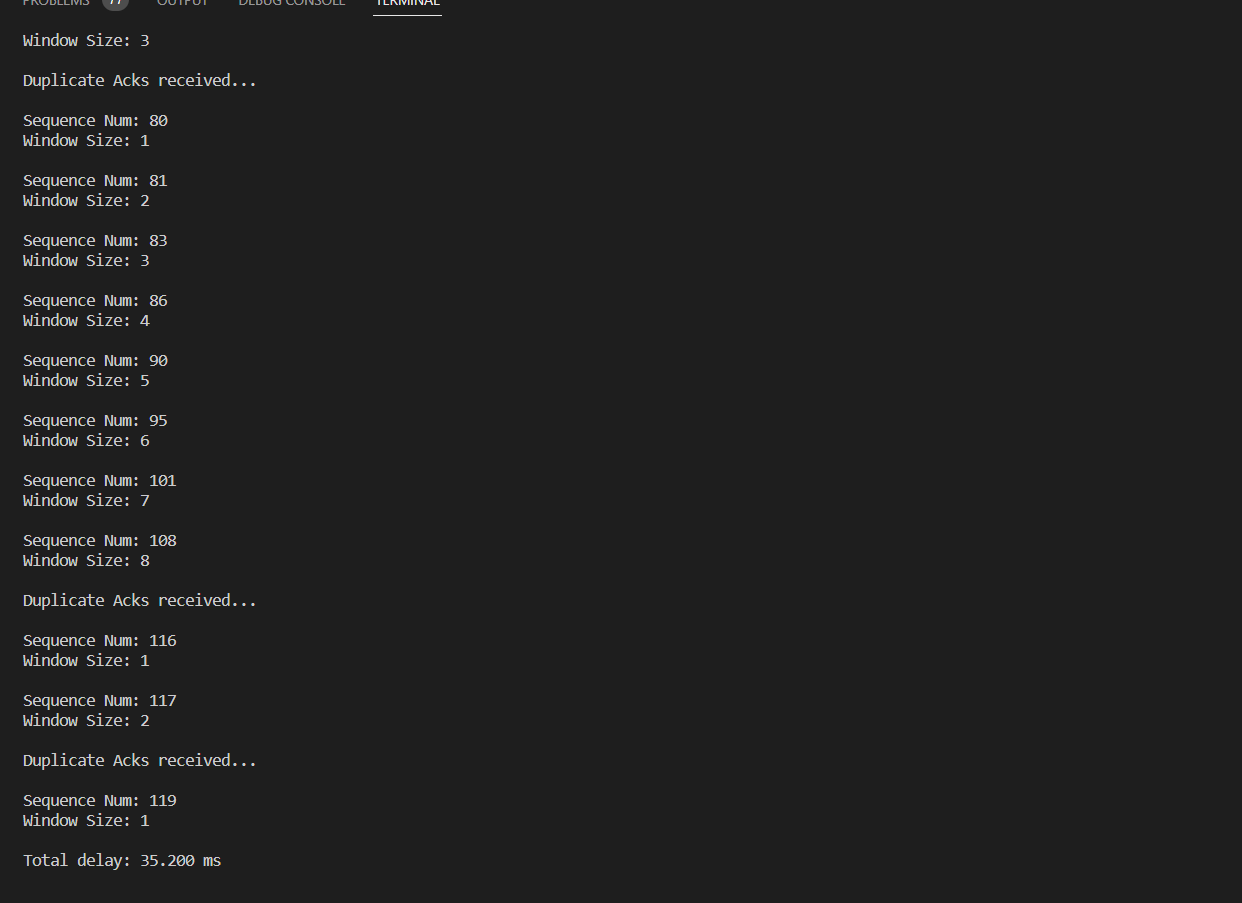
\includegraphics[width=\textwidth]{t_client3.png}
\caption{Terminal output of client java file }
\end{figure}
\FloatBarrier


\section{Comparison between TCP Reno and TCP Tahoe }
TCP Reno and TCP Tahoe are two variants of the Transmission Control Protocol (TCP) that are used for reliable data transmission over the internet. While both protocols use similar mechanisms for congestion control and flow control, there are some key differences between them:

1. Fast Recovery: The most significant difference between TCP Tahoe and TCP Reno is the way they handle packet loss. In TCP Tahoe, when a packet loss is detected, the congestion window is reduced to 1 and the slow start phase is entered. This means that the congestion window size is increased exponentially until the slow start threshold is reached, and then increased linearly.
In TCP Reno, a fast recovery phase is added. When a packet loss is detected, the congestion window is halved, and the fast recovery phase is entered. In this phase, the congestion window size is kept constant until all lost packets are retransmitted. After that, the congestion avoidance phase is entered, and the congestion window size is increased linearly.

2. Congestion Window Size: In TCP Tahoe, the congestion window size is reduced to 1 when a packet loss is detected. This can lead to a significant decrease in throughput, especially in high-bandwidth networks. 

In TCP Reno, the congestion window size is halved when a packet loss is detected. This means that the throughput is not reduced as much as in TCP Tahoe, and the network can recover more quickly from congestion.

In summary, the main difference between TCP Tahoe and TCP Reno is the way they handle packet loss. Figure 4 illustrates the evolution of TCP’s congestion window for both TCP Tahoe and Reno.

  \begin{figure}[!h]
\centering
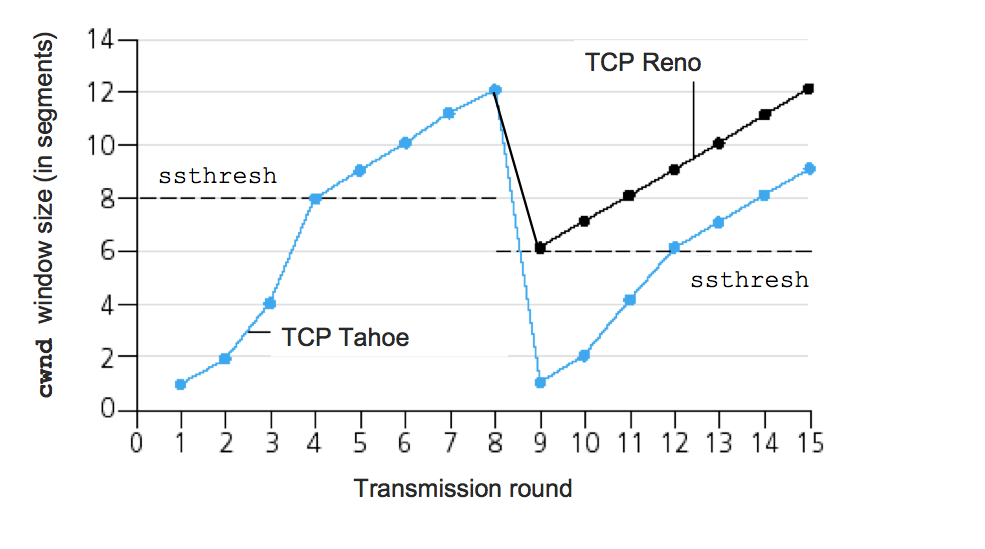
\includegraphics[width=\textwidth]{tahoe-reno.png}
\caption{Evolution of TCP's Congestion Window[Tahoe and Reno]  }
\end{figure}
\FloatBarrier

In this figure, the threshold is initially equal to 8 MSS. For the first eight transmission rounds, Tahoe and Reno take identical actions. The congestion window climbs exponentially fast during slow start and hits the threshold at the fourth round of transmission. The congestion window then climbs linearly until a triple duplicate- ACK event occurs, just after transmission round 8. Note that the congestion window is 12 MSS when this loss event occurs.

The value of ssthresh is then set to 0.5 *cwnd = 6 MSS. Under TCP Reno, the congestion window is set to cwnd = 9 MSS and then grows linearly. Under TCP Tahoe, the congestion window is set to 1 MSS and grows exponentially until it reaches the value of ssthresh, at which point it grows linearly.


4. Retransmission: TCP Reno allows for selective retransmission, meaning that only the lost packets are retransmitted, while the rest of the packets are not affected. This can help to improve the efficiency of transmission, as retransmitting all packets can be wasteful. TCP Tahoe, on the other hand, uses a more conservative approach of retransmitting all packets that have not been acknowledged.

5. Performance: In general, TCP Reno performs better than TCP Tahoe in congested network environments. Reno is able to more quickly detect and respond to congestion, which can help to avoid network congestion and improve the overall throughput. However, in non-congested network environments, TCP Tahoe can perform just as well as TCP Reno.

In summary, TCP Reno and TCP Tahoe are both reliable data transmission protocols that use similar mechanisms for congestion control and flow control. However, TCP Reno is generally considered to be a more advanced protocol, as it uses more aggressive congestion avoidance mechanisms and has a faster recovery mechanism for lost packets. As a result, TCP Reno is often preferred over TCP Tahoe in congested network environments.


\section{Experience}
In the lab report on "Implementation of TCP Reno congestion control algorithm," we conducted a comprehensive study on the implementation of TCP Reno. Through this, we got a better understanding of how not to overwhelm the receiver with more data than it can handle and how to prevent congestion in the network. 



\begin{thebibliography}{1}
\bibitem{book}  Computer networking : a top-down approach 6th ed.
\bibitem{StackOverflow} StackOverflow : \url{http://stackoverflow.com/}
\bibitem{Geeks for geeks} GeeksforGeeks : \url{https://www.geeksforgeeks.org/}
\end{thebibliography}

\end{document}